\chapter{Introduction}
\label{chap:Introduction}

\section{Motivation}

Modern rail vehicles like trains, metro vehicles or trams have to meet ever increasing acoustic requirements and strict noise legislation not only to improve the acoustic comfort of the passengers, but also to reduce environmental noise pollution caused by the railway transportation \cite{paozalyte_pollution_2011, li_25d_2021, zhang_sound_2019}.
% source of railway noise
A significant part of the train noise comes from the vehicle underfloor area, where the bogies and auxiliary equipment, for example, the air supply system, the hydraulic system, or the electric system, are located. The major source of the underfloor noise is the rolling noise emitted by the wheel-rail interface at the bogie area \cite{LUNDEN20093}. Besides that, for a driven bogie, the operational noise of traction motors also has a great contribution to the overall underfloor noise level\cite{Noh_2017, zhang_sound_2019}.
% transmission of the underfloor noise
The bogie area noise can be transmitted into the car interior through both structure-borne and airborne path as depicted in \cref{fig:transmission_path}. The structure-borne component of the bogie area noise is mainly due to the vibrations of the wheel that are transmitted through the car suspension into the vehicle interior. 
The airborne component, on the one hand, propagates directly into the exterior of the vehicle, disturbing the people in the surroundings, on the other hand, it could also be transmitted into the car interior for example through windows and doors, affecting the comfort of the passenger.
%
Hence, having a computational model that can assess the underfloor noise already in the early development phase of the rail vehicle is of great importance and can help in controlling both car exterior and interior noises.

\begin{figure}
	\centering
	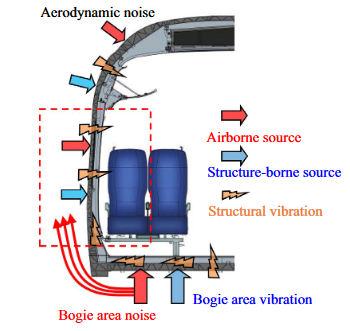
\includegraphics[width=0.5\textwidth]{fig/noise_transmission_path.png}
	\caption{Transmission path of exterior noise sources. Figure taken from \cite{zhang_sound_2019}.}
	\label{fig:transmission_path}
\end{figure}


\section{Aims and objectives}

This thesis, conducted in collaboration with Siemens Mobility Austria GmbH, focuses on the propagation of the underfloor noise into the railway vehicle's surroundings and aims to develop a computational model that can predict the pressure field distribution around the vehicle car body due to the bogie area noise, based on the finite element method (FEM).
The modeling approach should be applied to the metro train type X-Wagen from Siemens and an artificial noise source beneath the underframe should be used as excitation.
Furthermore, the finite element model is to be validated by an outer pressure field measurement with the vehicle at standstill, which is also a part of this thesis.
The developed finite element model in the framework of this thesis should provide a good starting point for the further modeling using the finite element method for the underfloor noise prediction and should answer the following main research questions and tasks:
\begin{itemize}
	\item Develop a simulation workflow of the underfloor noise prediction using FEM.
	\item What are the necessary boundary conditions and how can they be incorporated into the finite element model?
	\item How much of the vehicle and its surroundings can be considered in the model with currently available computational resources?
	\item How accurate is the prediction of the model and how sensitive are the simulation results with respect to several parameter variations?
	\item Assess the applicability of the modeling approach using FEM and determine its limitations.
\end{itemize}

\section{Structure of the thesis}

The remainder of this thesis is organized as follows. First, \cref{chap:Theory} provides a fundamental background of the thesis. In the chapter, the governing equations and the finite element formulation of the linear acoustic problem are explained, the perfectly matched layer (PML) technique to simulate acoustic open domain is introduced, and important terminologies from the noise measurement technique are summarized. Further, this chapter also gives a brief overview of the metro train type X-Wagen, on which the finite element modeling approach will be applied. In \cref{chap:measurement}, the sound power measurement of the omnidirectional noise source serving as the input for the finite element simulation is carried out. Further, the outer pressure field distribution in the vehicle surroundings due to an artificial noise source beneath the car floor is measured and will be later used as validation for the finite element model. \Cref{chap:FEM} describes the design and development of the finite element model. A parameter study is carried out to find an optimal simulation domain size of the acoustic open region. A modeling approach of the sound source is introduced to incorporate the measured input sound power into the finite element model. Further, besides the initial simulation setup for the underfloor noise prediction, several parameter studies on different model parameters are also prepared to investigate the solution sensitivity. In \cref{chap:results}, the obtained simulation results are compared with the validation measurement to validate the finite element model. Consequently, the obtained results from the parameter studies are also presented. Finally, \cref{chap:summary} summarizes the thesis and provides an outlook on possible adaptions and extensions to the performed simulations and lists the future work.
